\section{Đánh giá kết quả}

\subsection{Khung đánh giá chất lượng mô hình}

Chất lượng mô hình được theo dõi bằng ba chỉ số chuẩn cho hồi quy: MAE, RMSE và $R^2$. Ba chỉ số này được tính trên tập test sau phép chia train-test 80/20 và được ghi lại trong metadata của mỗi version mô hình. Phần định nghĩa toán học, ý nghĩa của từng ký hiệu và lập luận lựa chọn bộ ba chỉ số này đã được trình bày ở Mục 2.4. Trong chương này, ba chỉ số được sử dụng như khung đánh giá thực nghiệm thống nhất để so sánh các version mô hình trong kho hiện hành.
\subsection{So sánh tổng quan các version mô hình}

Ở giai đoạn đánh giá, từng model không được xem như một artifact độc lập mà được đặt trong cùng một không gian thực nghiệm. Vì vậy, trước khi đi vào phân tích chi tiết một version cụ thể, cần nhìn toàn bộ các model hiện hành như một chuỗi thí nghiệm, trong đó mỗi version phản ánh một lựa chọn khác nhau về dữ liệu, tập feature hoặc cấu hình huấn luyện.

\blockparagraph{Tiêu chí so sánh}

Việc so sánh các version được thực hiện trên cùng ba chỉ số MAE, RMSE và $R^2$. Trong giao diện quản trị hiện tại, tiêu chí xếp hạng chính để gợi ý ``best choice'' là $R^2$ cao nhất; tuy nhiên, trong phân tích, cả ba chỉ số vẫn cần được đọc đồng thời để tránh kết luận thiên lệch theo một thước đo duy nhất.

\blockparagraph{Bảng tổng hợp các version hiện hành}

\begin{center}
\begin{tabular}{|c|c|c|c|c|c|}
\hline
\textbf{Version} & \textbf{Records} & \textbf{Features} & \textbf{$R^2$} & \textbf{MAE} & \textbf{RMSE} \\
\hline
v1 & 3567 & 6 & 0.9217 & 23.1648 & 39.6847 \\
\hline
v2 & 3568 & 6 & 0.8954 & 21.5228 & 37.3287 \\
\hline
v3 & 4454 & 6 & 0.9556 & 34.7660 & 60.2850 \\
\hline
v4 & 4454 & 8 & 0.9610 & 31.8551 & 54.9547 \\
\hline
v5 & 3454 & 8 & 0.6983 & 19.1244 & 28.4388 \\
\hline
\end{tabular}
\end{center}

\begin{figure}[H]
    \centering
    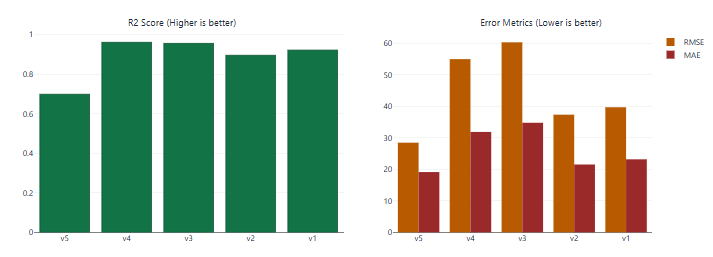
\includegraphics[width=0.88\textwidth]{graphics/result.png}
    \caption{Đồ thị tổng hợp các chỉ số đánh giá chất lượng của các version mô hình.}
\end{figure}

Bảng trên cho thấy các version hiện tại không tạo thành một trật tự đơn điệu trên mọi chỉ số. Nếu xét theo $R^2$, \texttt{v4} là phiên bản tốt nhất; nếu xét theo MAE và RMSE, \texttt{v5} lại có sai số tuyệt đối thấp hơn. Điều này cho thấy việc đánh giá mô hình trong hệ thống phải được hiểu như một bài toán đa tiêu chí, thay vì một phép xếp hạng tuyến tính đơn giản.

Theo tiêu chí xếp hạng đang được dashboard sử dụng, phiên bản được đánh giá tốt nhất trong kho model hiện hành là \texttt{v4}, tức version có $R^2$ cao nhất. \texttt{v4} được chọn làm đối tượng phân tích trọng tâm vì đây là model thể hiện tốt nhất khả năng nắm bắt cấu trúc biến thiên của dữ liệu mục tiêu trên tập đánh giá.

Về mặt định lượng, đây là version có mức giải thích phương sai cao nhất trong toàn bộ kho model hiện tại.

\begin{itemize}
    \item \textbf{Về khả năng giải thích dữ liệu:} $R^2 \approx 0.961$ cho thấy mô hình đã học được phần lớn cấu trúc biến thiên của giá trên tập test. Đây là cơ sở chính để \texttt{v4} được dashboard xếp ở vị trí tốt nhất.
    \item \textbf{Về nguyên nhân cải thiện:} so với các version trước, \texttt{v4} hưởng lợi từ hai thay đổi quan trọng là tập dữ liệu lớn hơn và feature set được mở rộng từ 6 lên 8 biến. Hai biến bổ sung là \texttt{release\_year} và \texttt{days\_used} đưa thêm thông tin về vòng đời và mức khấu hao của thiết bị.
    \item \textbf{Về giới hạn của kết quả:} \texttt{v4} không phải model có MAE hay RMSE thấp nhất. Điều này cho thấy khả năng giải thích phương sai tổng thể và độ lớn sai số tuyệt đối không hoàn toàn đồng biến trong các thí nghiệm hiện có, \texttt{v4} được xem là model tốt nhất theo tiêu chí xếp hạng hiện hành của hệ thống, chứ chưa thể xem là phiên bản tối ưu tuyệt đối trên mọi góc nhìn đánh giá.
\end{itemize}

\blockparagraph{Tầm quan trọng đặc trưng của version v4}

Metadata của \texttt{v4} cho thấy thứ tự feature importance giảm dần là: \texttt{brand}, \texttt{storage}, \texttt{screen\_size}, \texttt{release\_year}, \texttt{battery\_capacity}, \texttt{ram}, \texttt{days\_used}, \texttt{camera\_mp}.

\begin{itemize}
    \item \textbf{Nhóm tác động mạnh nhất:} \texttt{brand} đứng đầu, cho thấy dữ liệu thị trường hiện tại vẫn mang dấu ấn thương hiệu rất rõ trong quá trình hình thành giá.
    \item \textbf{Nhóm phân khúc kỹ thuật:} \texttt{storage}, \texttt{screen\_size} và \texttt{ram} giúp mô hình phân biệt các cụm thiết bị theo cấu hình và phân khúc sử dụng.
    \item \textbf{Nhóm vòng đời sản phẩm:} \texttt{release\_year} và \texttt{days\_used} bổ sung thông tin trực tiếp về thế hệ sản phẩm và mức khấu hao theo thời gian.
    \item \textbf{Nhóm giá trị sử dụng thực tế:} \texttt{battery\_capacity} và \texttt{camera\_mp} không phải các biến chi phối mạnh nhất, nhưng vẫn góp phần phản ánh chất lượng sử dụng và sức hấp dẫn của thiết bị trên thị trường.
    \item \textbf{Nhận xét tổng quát:} mô hình không chỉ học từ thông số phần cứng, mà còn khai thác được đồng thời tín hiệu thương hiệu, vòng đời công nghệ và mức độ hao mòn của sản phẩm.
\end{itemize}

\subsection{Thảo luận kết quả}

Sau khi đặt các version vào cùng một khung so sánh và chọn ra model được đánh giá tốt nhất theo tiêu chí hiện hành, bước tiếp theo là diễn giải kết quả trong bối cảnh vận hành của hệ thống. Mục tiêu ở đây không chỉ là trả lời ``model nào tốt hơn'', mà còn là làm rõ hệ quả của các kết quả đó đối với việc triển khai và sử dụng mô hình trong ứng dụng.

\blockparagraph{Ý nghĩa của việc so sánh version}

Cơ chế so sánh version cho phép trả lời các câu hỏi thực nghiệm cốt lõi: mở rộng feature set có giúp cải thiện mô hình hay không, tăng dữ liệu tổng hợp có thực sự nâng chất lượng, và thay đổi cấu hình huấn luyện tác động ra sao đến từng chỉ số. Nhờ đó, quá trình phát triển model được tổ chức như một chuỗi thí nghiệm có kiểm soát, thay vì chỉ là tập hợp các lần train rời rạc.

\blockparagraph{Ý nghĩa đối với quyết định triển khai}

Kết quả hiện tại cho thấy việc chọn model để phục vụ runtime không nhất thiết trùng với model có $R^2$ cao nhất. Đây là một điểm quan trọng trong thiết kế hệ thống: môi trường vận hành có thể ưu tiên một version ổn định hơn theo sai số tuyệt đối hoặc phù hợp hơn với phân phối dữ liệu đang khai thác, trong khi môi trường đánh giá học thuật có thể ưu tiên version có năng lực giải thích mạnh hơn về mặt thống kê.

\blockparagraph{Phạm vi sử dụng của kết quả hiện tại}

Trong trạng thái hiện tại, pipeline đã bao quát các lớp chính gồm dữ liệu, huấn luyện, versioning, dashboard quản trị và suy luận trực tiếp. Kết quả của mô hình được dùng như công cụ hỗ trợ tham chiếu giá, chưa được đặt như một cơ chế quyết định hoàn toàn tự động. Cách đặt phạm vi sử dụng như vậy phù hợp với bản chất của bài toán định giá khi dữ liệu vẫn còn giới hạn và nhiều biến ngữ cảnh chưa được đưa vào mô hình.
